%%%%%%%%%%%%%%%%%%%%%%%%%%%%%%%%%%%%%%%%%%%%%%%%%%%
%
%  Author: Jacob Vaughn
%  
%  Last Updated: 3/8/2024
%
%%%%%%%%%%%%%%%%%%%%%%%%%%%%%%%%%%%%%%%%%%%%%%%%%%%

%%%%%%%%%%%%%%%%%%%%%%%%%%%%%%%%%%%%%%%%%%%%%%%%%%%%%%%%%%%%%%%%%%%%%%%
%%%               DESIGN AND FABRICATION OF ACE2.0
%%%%%%%%%%%%%%%%%%%%%%%%%%%%%%%%%%%%%%%%%%%%%%%%%%%%%%%%%%%%%%%%%%%%%%


\chapter{DESIGN AND FABRICATION OF ACE2.0}

\section{Background and Motivation}

The existing ACE (Actively Controlled Expansion) tunnel was designed and manufactured between 2009 and 2010 and began operating in 2010 \cite{ace09,ace10-calibrate,tichenor-dis}. The ACE tunnel nozzle is 40 inches long from the throat to the test-section entrance. The test section is 14 inches wide and 9 inches tall. By varying throat height, the test-section Mach number can be varied from M = 5 to 8.

\subsection{ACE Turbulent Transition}

Below a unit Reynolds number of $Re/m = U/\nu \approx 3 \times 10^6 m^{-1}$ the rms pressure fluctuations in the test section are low, less than 1\%. At higher Re/m values, pressure fluctuation levels increase when the unit Reynolds number increases above $Re/m \approx 3 \times 10^6 m^{-1}$ \cite{aceturb}. It is desired to increase the unit Reynolds number at which laminar flow can be maintained. This document summarizes the hypothesis and supporting data regarding the pressure fluctuation levels increase and how it might be delayed to higher unit Reynolds numbers.
More stuff

\subsubsection{ACE Nozzle Noise Surveys}

Three recent pitot surveys have been conducted in the ACE tunnel. The first by Mai (2014) revealed transition occurring around a unit Reynolds number of $3 \times 10^6 m^{-1}$, as shown in Figure \ref{fig:mai-survey}. The same result was found by Neel (2019) shown in Figure \ref{fig:neel-survey} that transition occurs at this unit Reynolds number 6 inches upstream of the test section entrance. A final pitot survey in ACE by Wirth (2022) was conducted to determine whether the pressure fluctuation levels increase occurred at different Re/m values at positions farther upstream in the nozzle. He found pressure fluctuation levels increase at $Re' \approx 3 \times 10^6 m^{-1}$ at a measurement location 17 inches upstream of the test section entrance. His results in Figure \ref{fig:wirth-survey} align perfectly with Mai and Neel and clearly establish that the Reynolds number at which pressure fluctuation levels increase is not sensitive to location in the nozzle. This suggests that transition is not moving upstream through the nozzle as Reynolds number is increased.

\begin{figure}[ht]
    \centering
    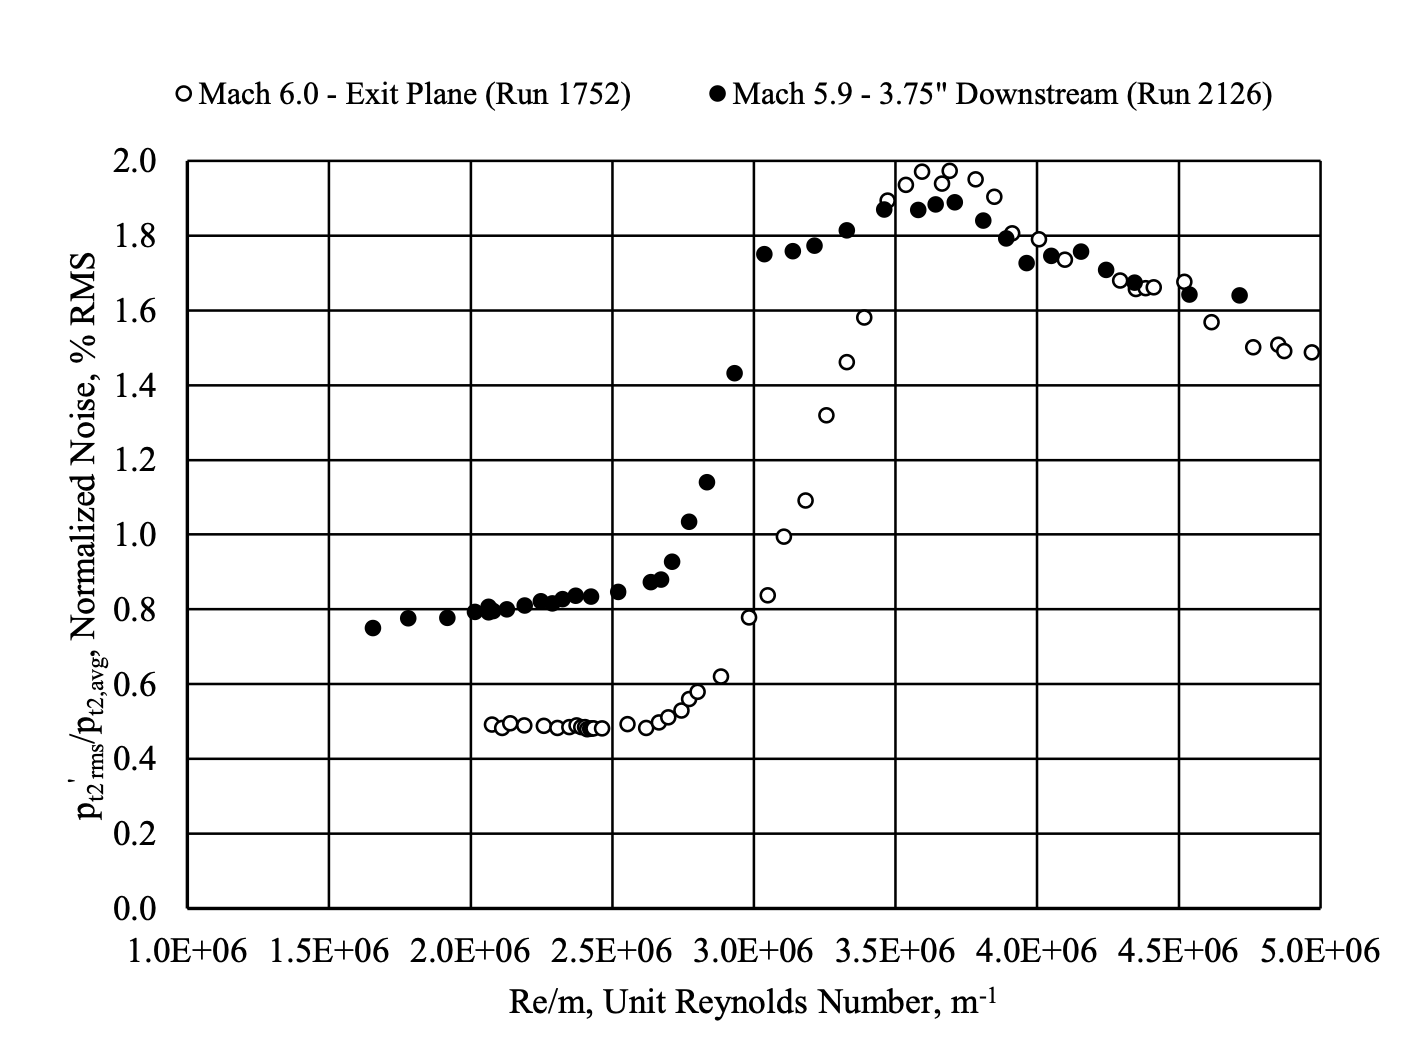
\includegraphics[width=6in]{mai-survey}
    \caption[ACE freestream pressure fluctuations at nozzle exit (2014)]{ACE freestream pressure fluctuations at nozzle exit (2014) \cite{mai-dis}}
    \label{fig:mai-survey}
\end{figure}

\begin{figure}[ht]
    \centering
    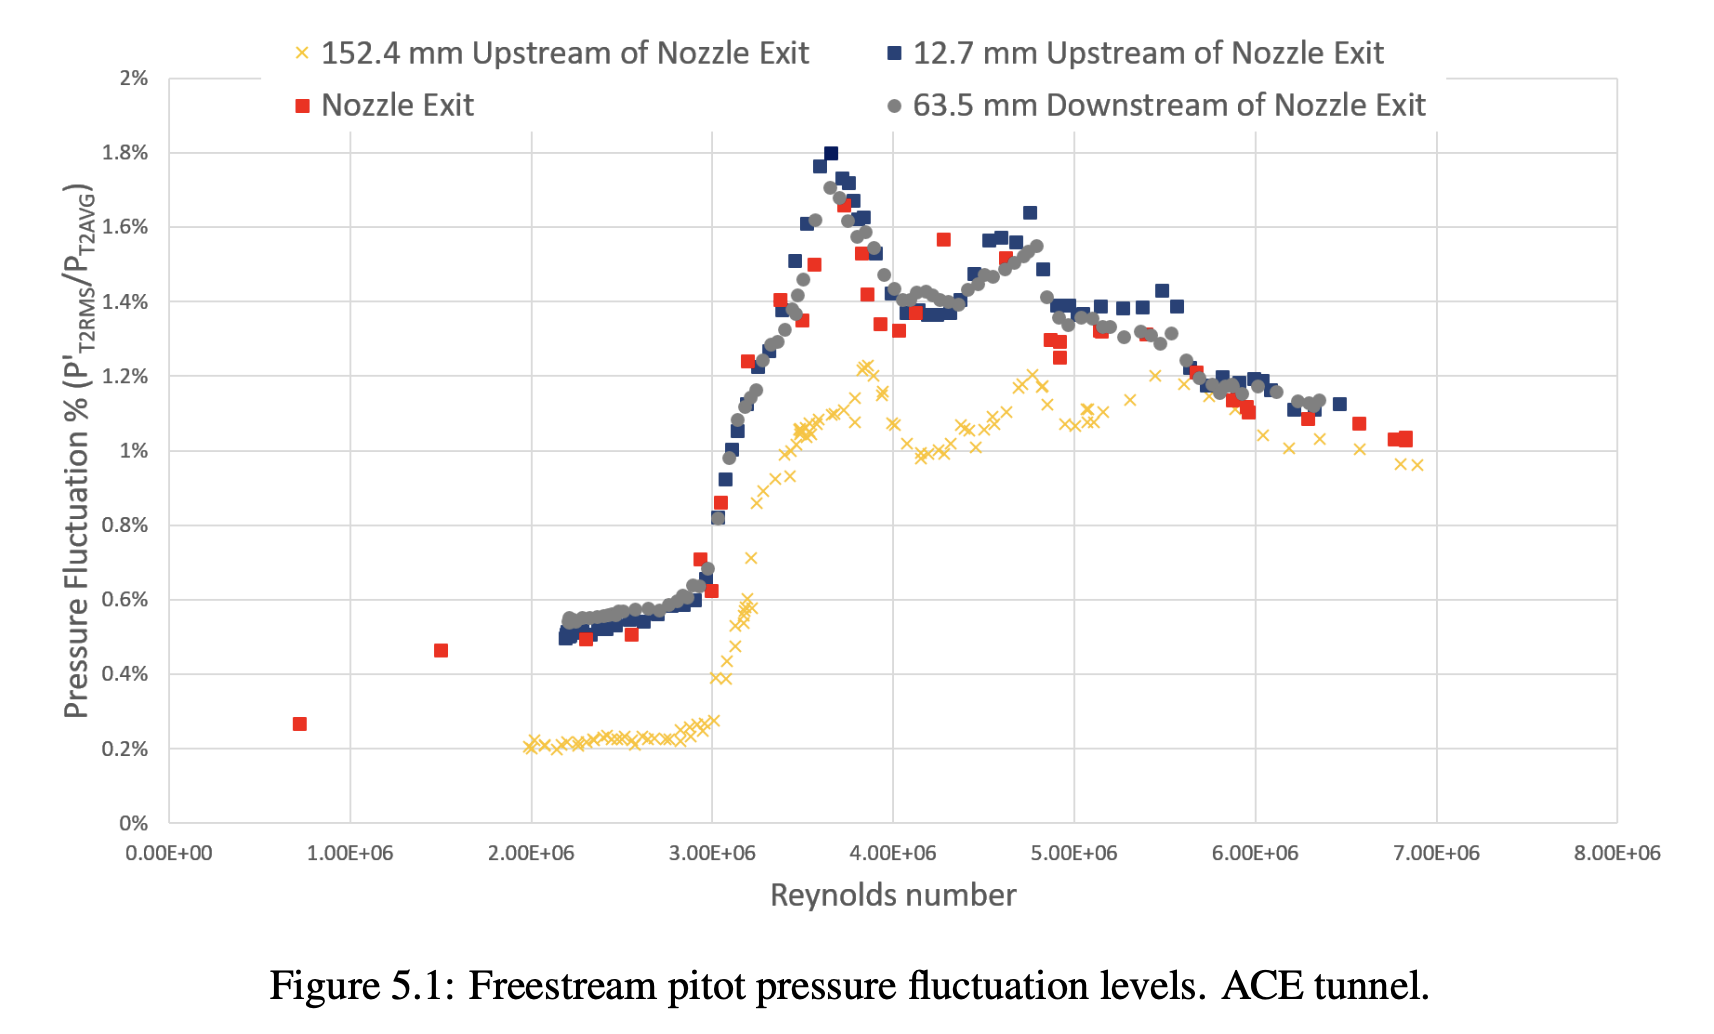
\includegraphics[width=6in]{neel-survey}
    \caption[ACE freestream pressure fluctuations at various locations (2019)]{ACE freestream pressure fluctuations at various locations (2019) \cite{neel-dis}}
    \label{fig:neel-survey}
\end{figure}

\begin{figure}[ht]
    \centering
    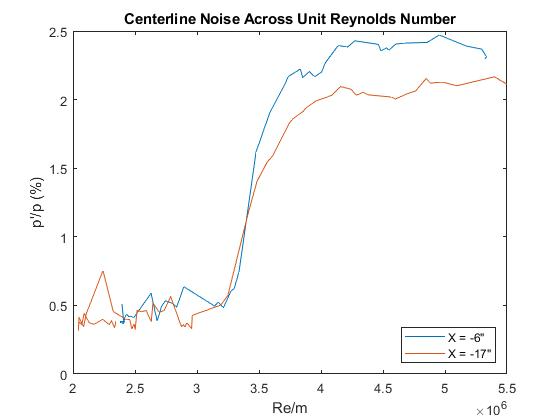
\includegraphics[width=6in]{wirth-survey}
    \caption{ACE freestream pressure fluctuations at 6 in. and 17 in. upstream of nozzle exit (2022)}
    \label{fig:wirth-survey}
\end{figure}

\subsubsection{Evaluation of Suspect Transition Mechanisms}

There are five primary suspects for this transition:

\begin{enumerate}
    \item A known manufacturing surface discontinuity at the throat
    \item Sidewall mushroom vortices
    \item Görtler vortices
    \item Freestream turbulence in the incoming flow and/or upstream boundary layer
    \item Wall roughness or waviness
\end{enumerate}

This following evaluates each of these possibilities and concludes that the primary culprit is the surface discontinuity at the throat. This conclusion is supported by pitot surveys, method-of-characteristics line tracing, and CFD simulations. Sidewall mushroom vortices and Görtler vortices would lead to transition too far downstream from the throat to be responsible for the pressure fluctuation levels increase. Items 4 and 5 are potential causes of poor flow quality in all supersonic tunnels and are included for completeness. The specific mechanism by which these would cause transition is not known. While they are not the primary suspects for the pressure fluctuation levels increase, improving these conditions will be addressed in the redesign intended to extend laminar flow to higher Reynolds numbers.

\subsubsection*{Mach Line Tracing}

The origin of the noise measured farthest upstream of the nozzle exit was determined by tracing characteristics from the measurement location at the centerline upstream to the wall. Both the side view and top view of this can be seen in Figure \ref{fig:machlines}.

\begin{figure}[ht]
    \centering
    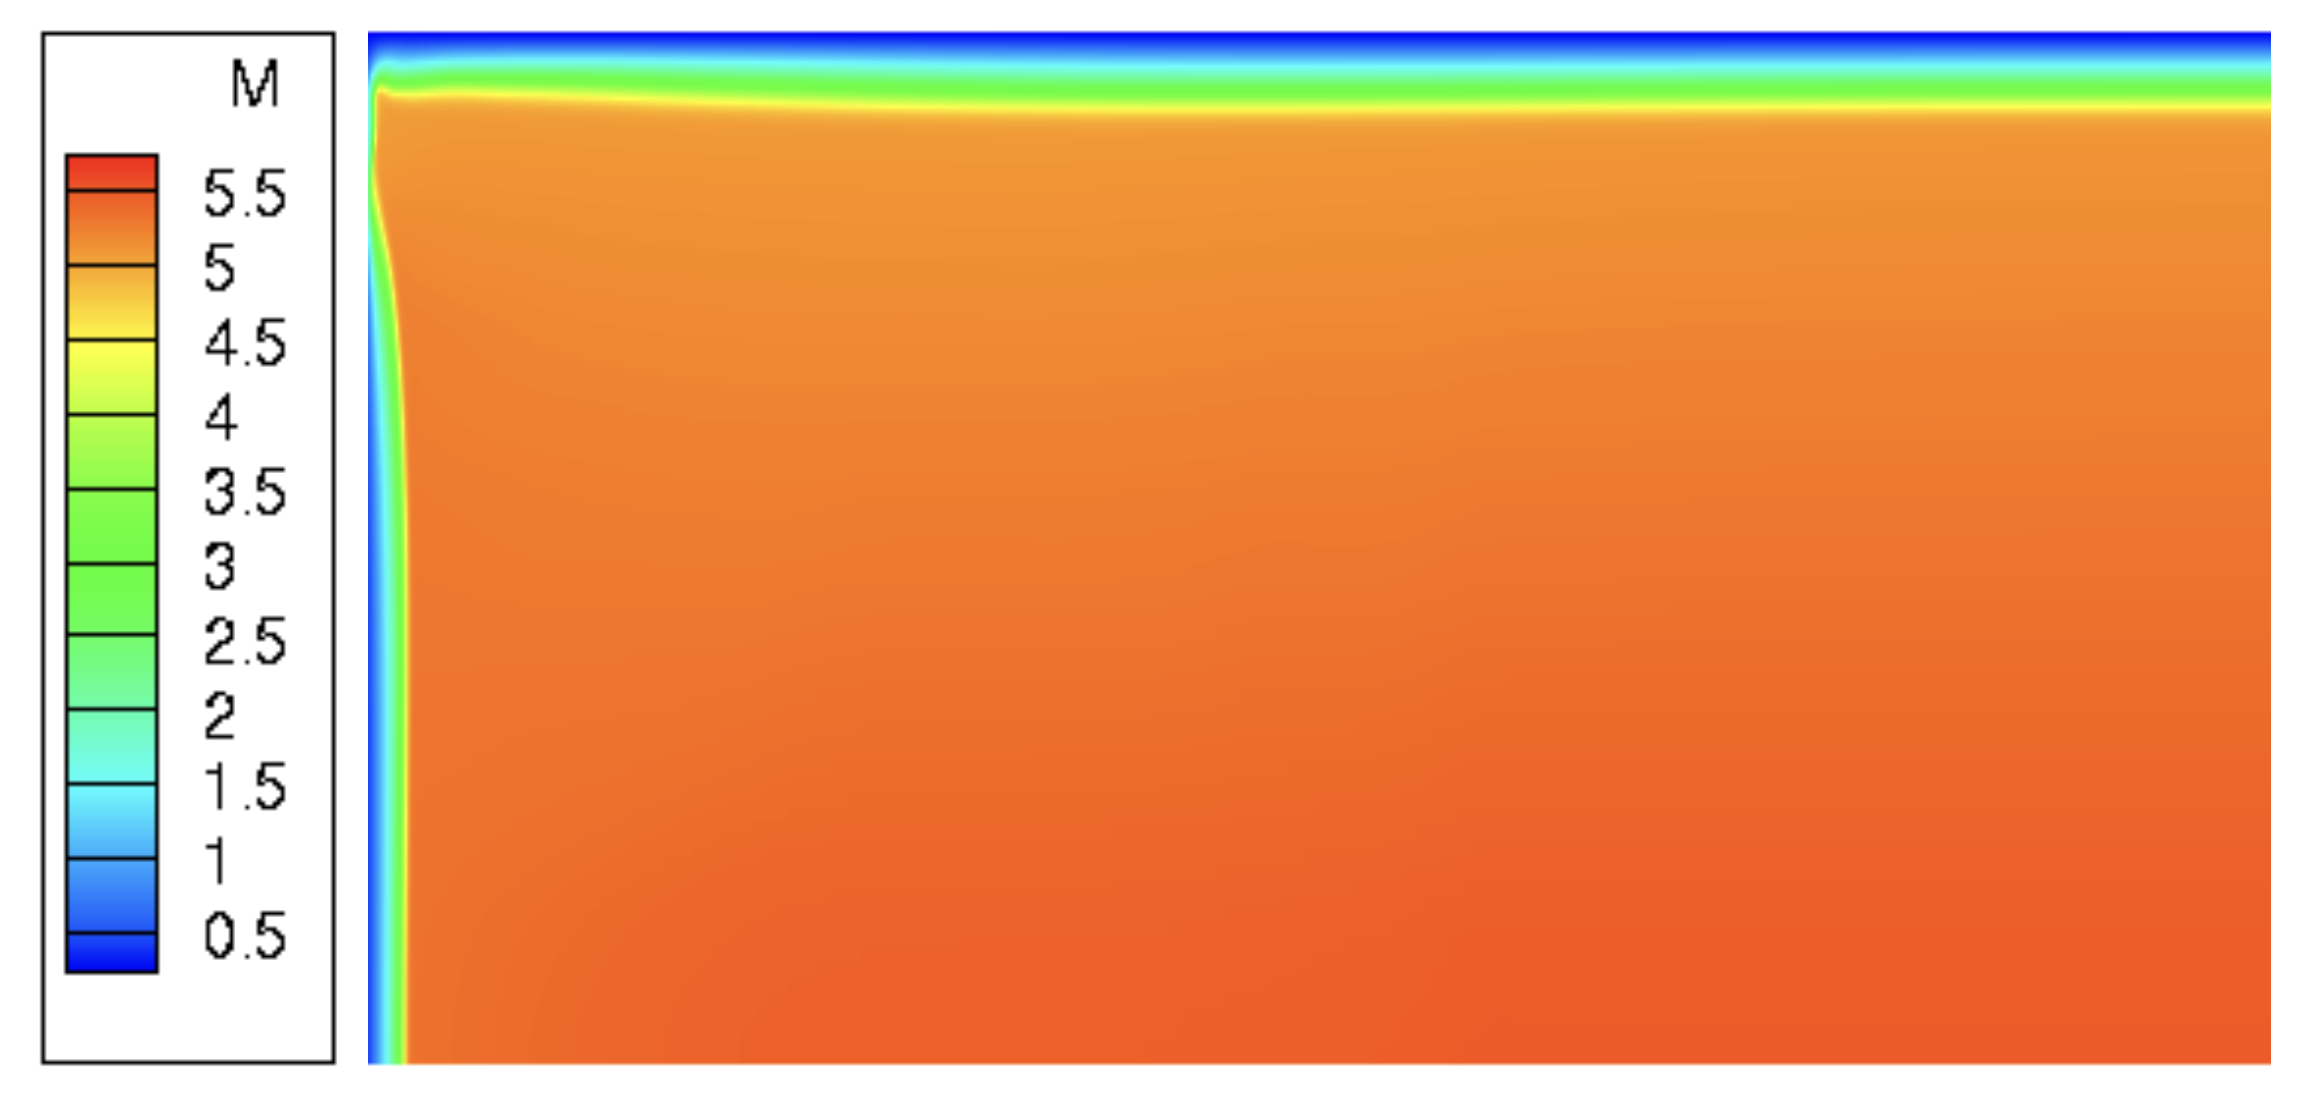
\includegraphics[width=6in]{mush24}
    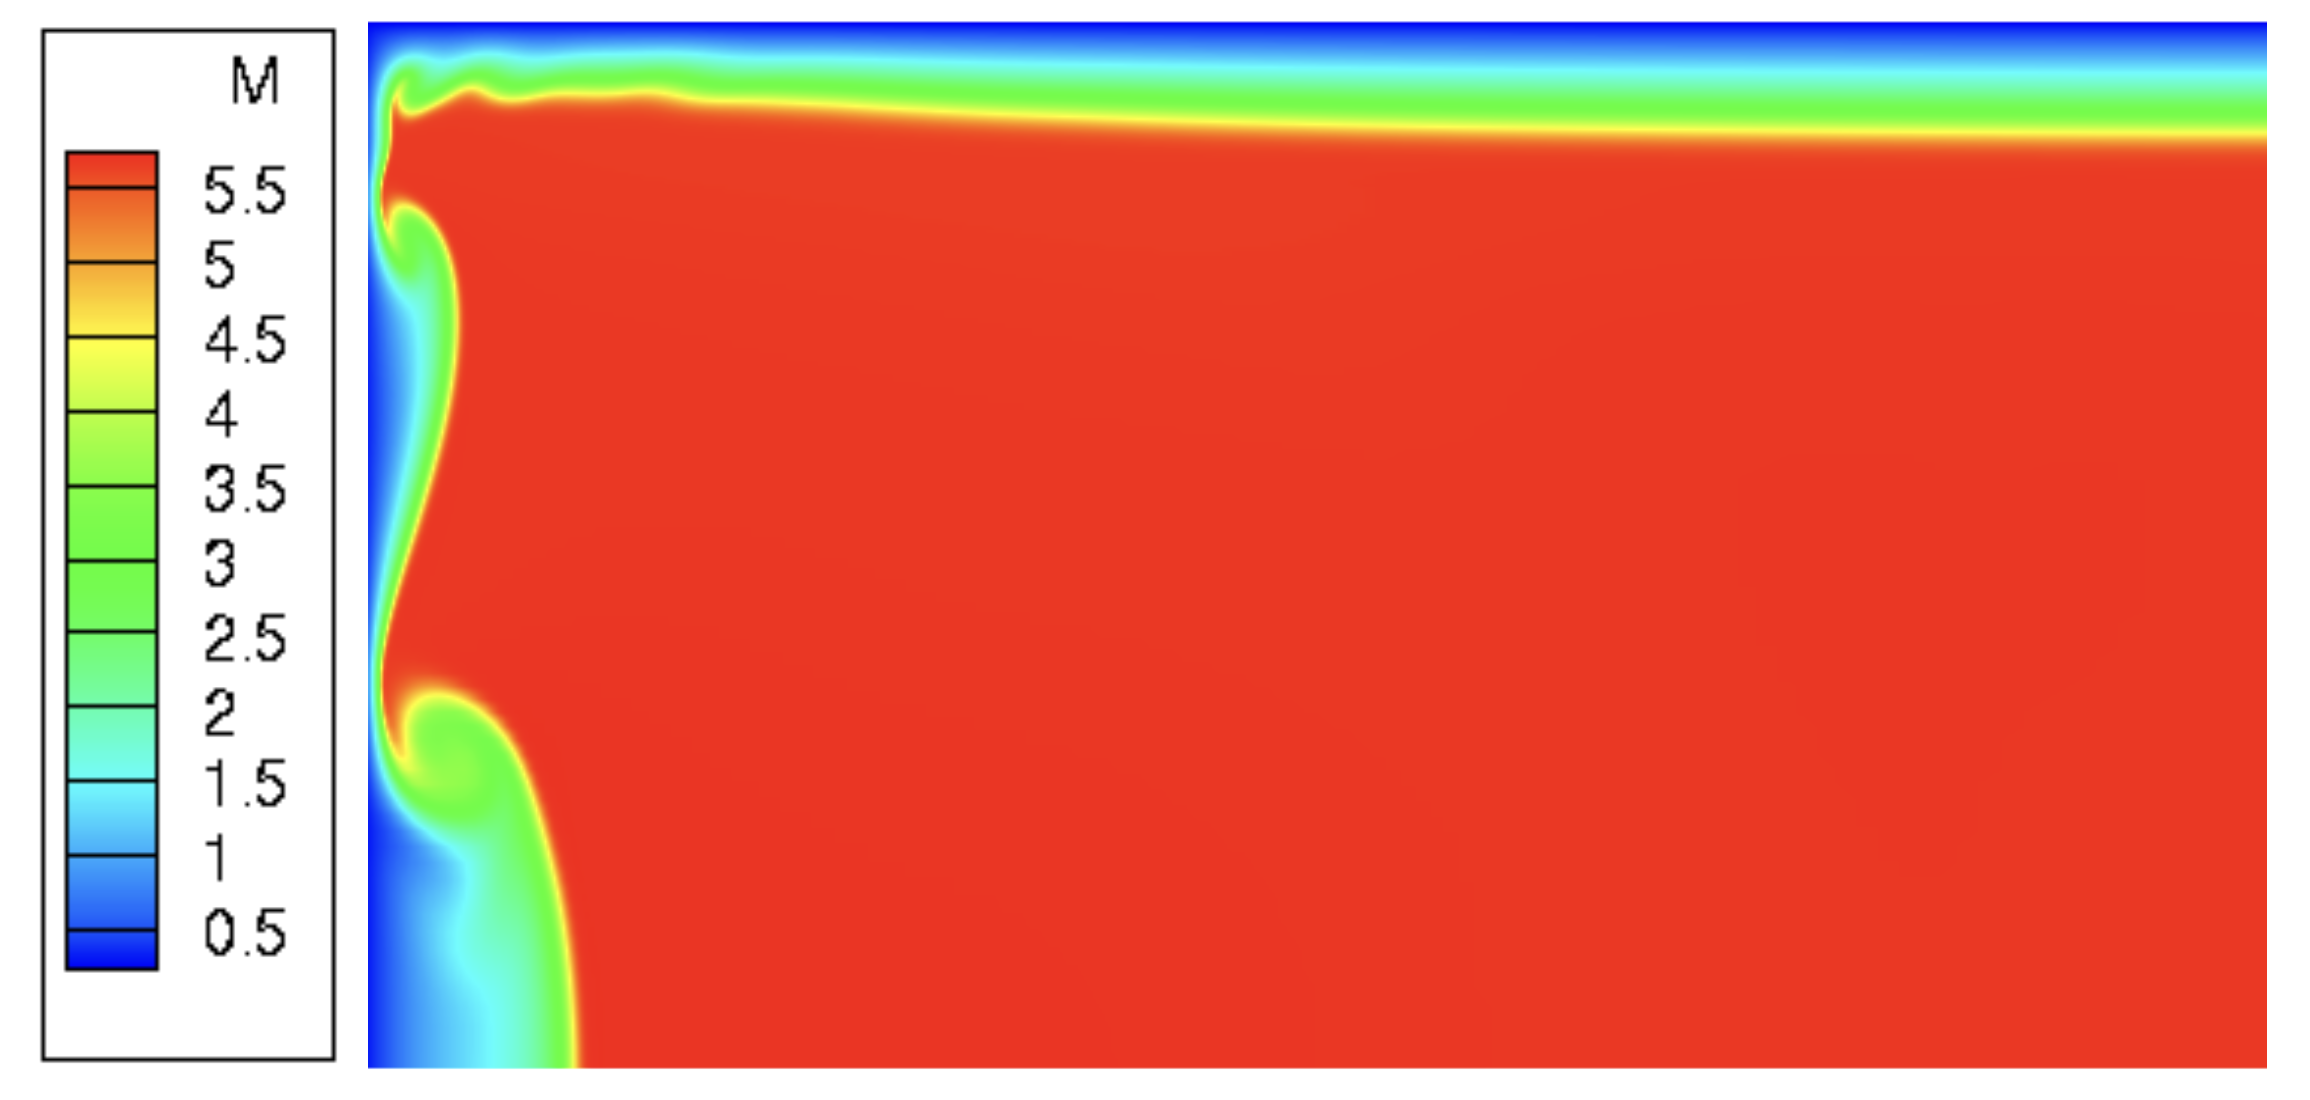
\includegraphics[width=6in]{mush0}
    \caption{Mushroom vortex formation at sidewalls}
    \label{fig:mushrooms}
\end{figure}

\begin{figure}[ht]
    \centering
    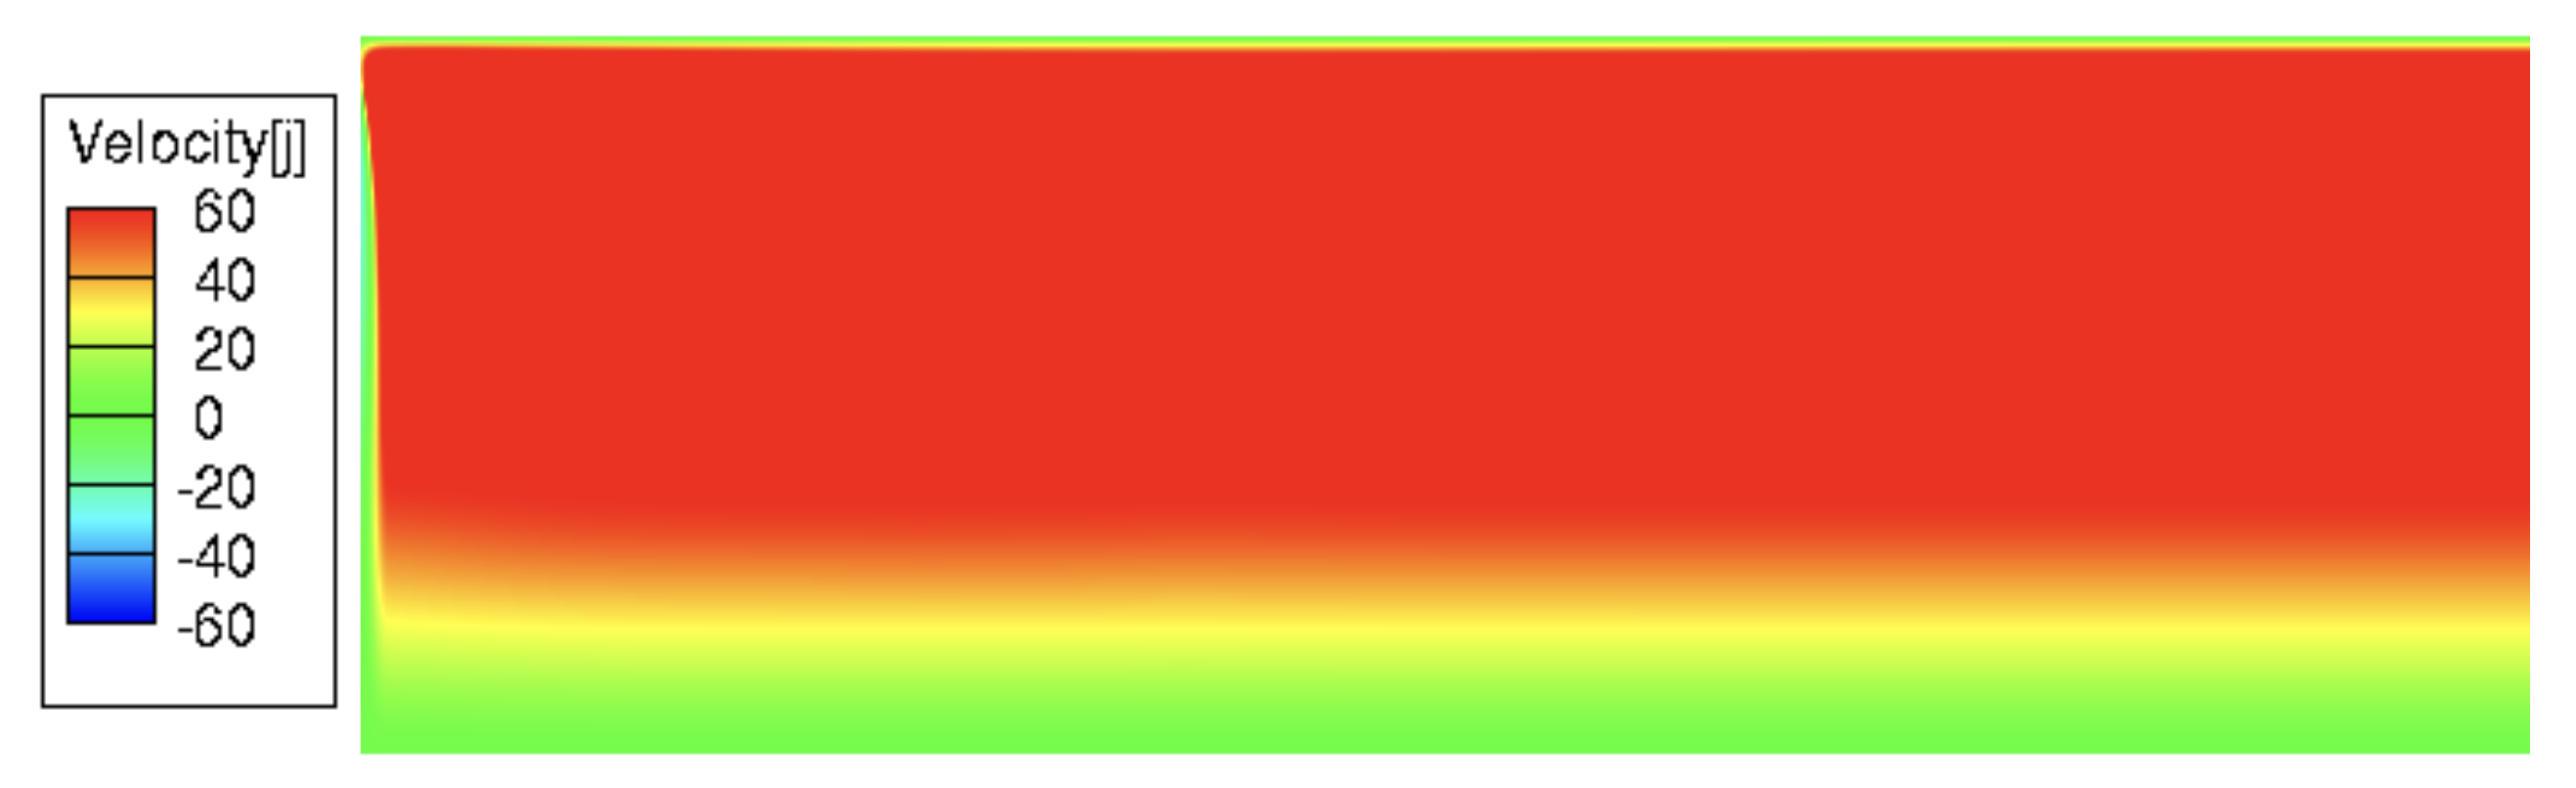
\includegraphics[width=6in]{vertical28}
    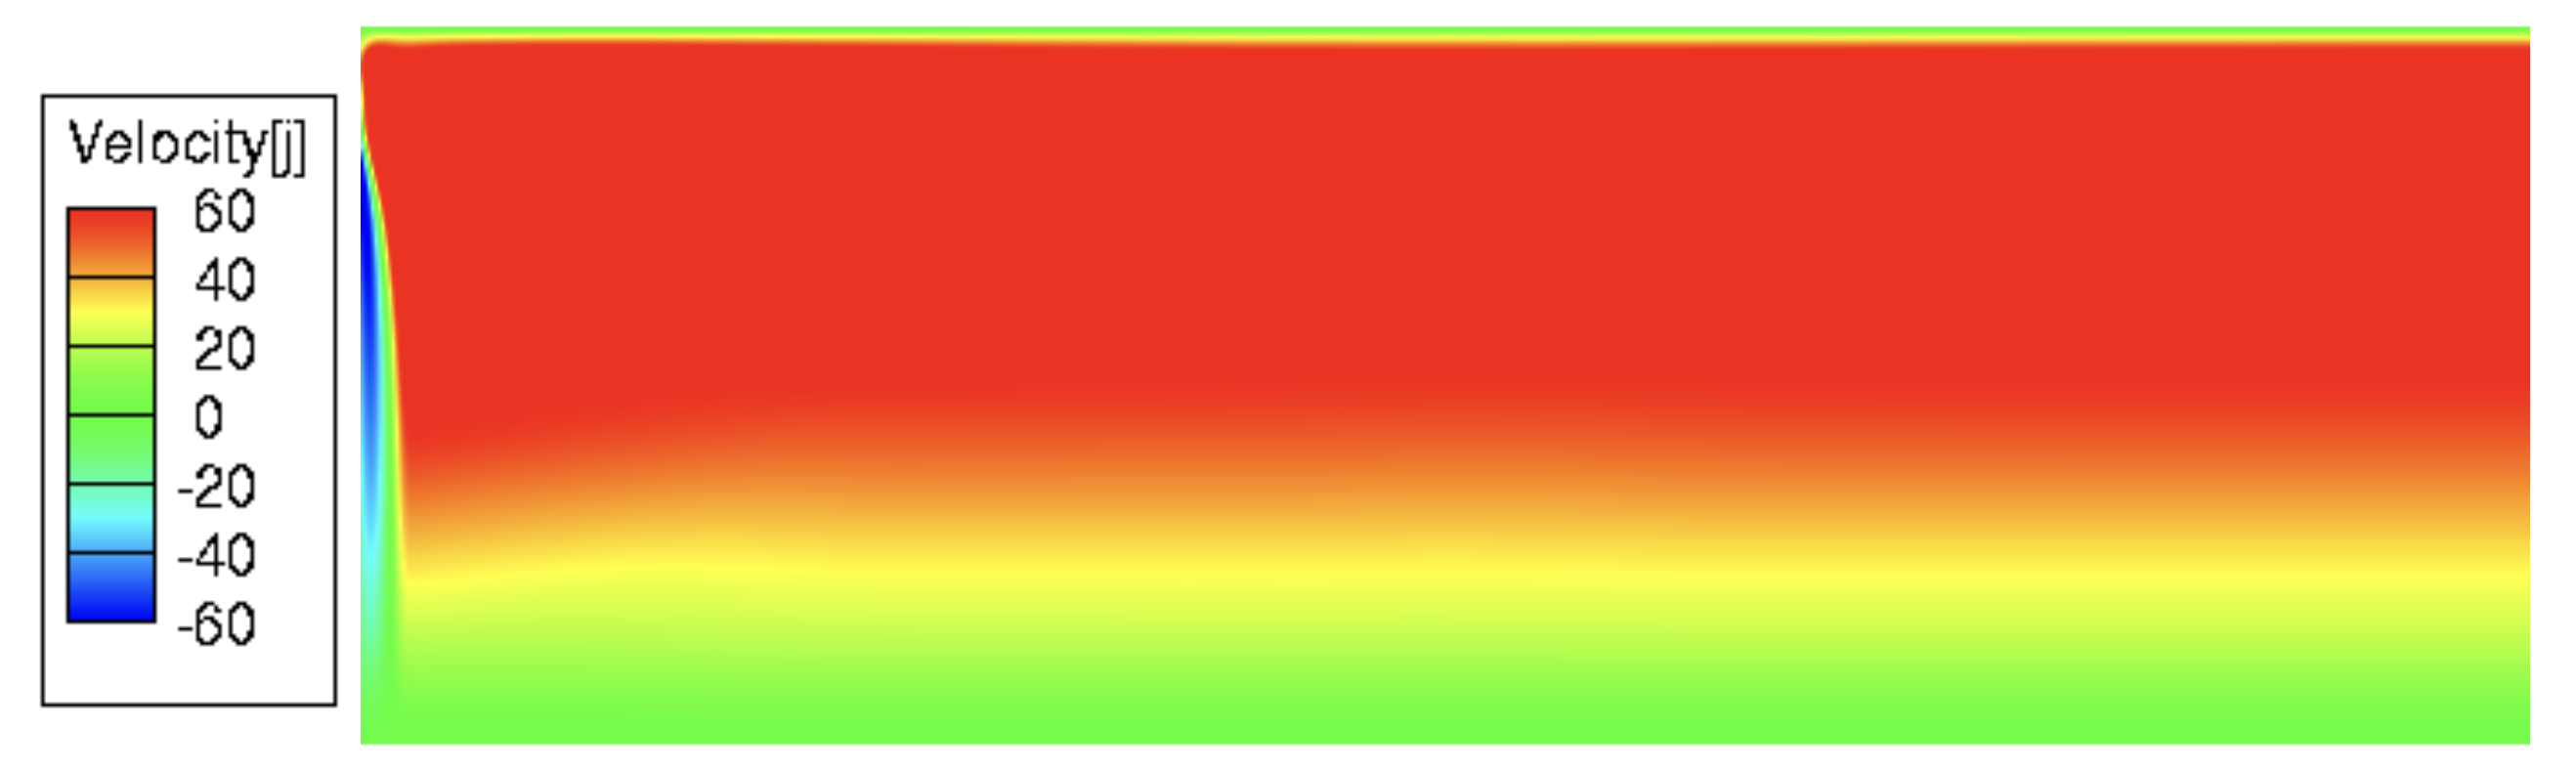
\includegraphics[width=6in]{vertical24}
    \caption{Vertical velocity}
    \label{fig:vertical-vel}
\end{figure}

\begin{figure}[ht]
    \centering
    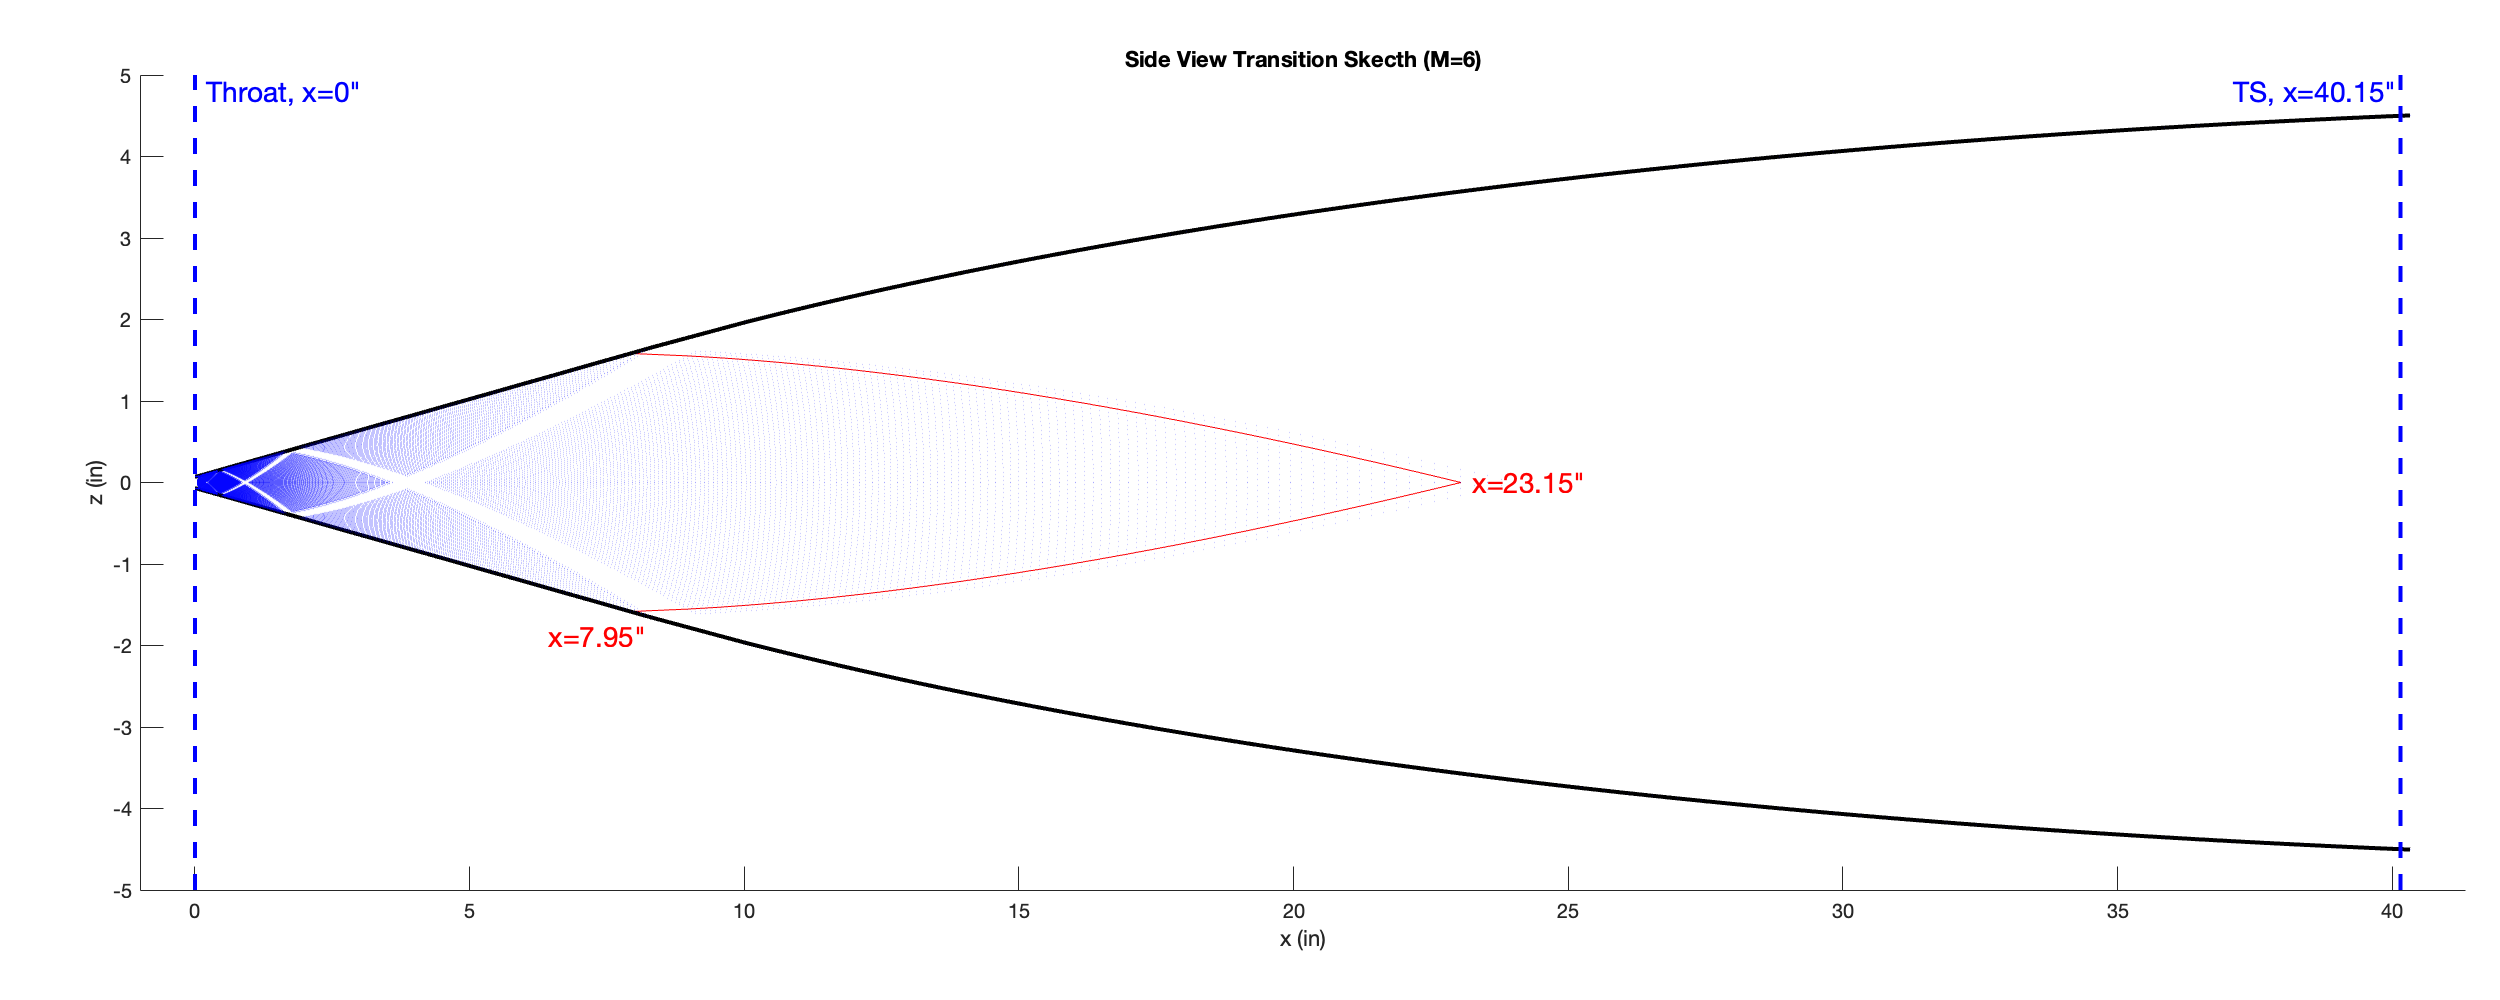
\includegraphics[width=6.5in]{side17}
    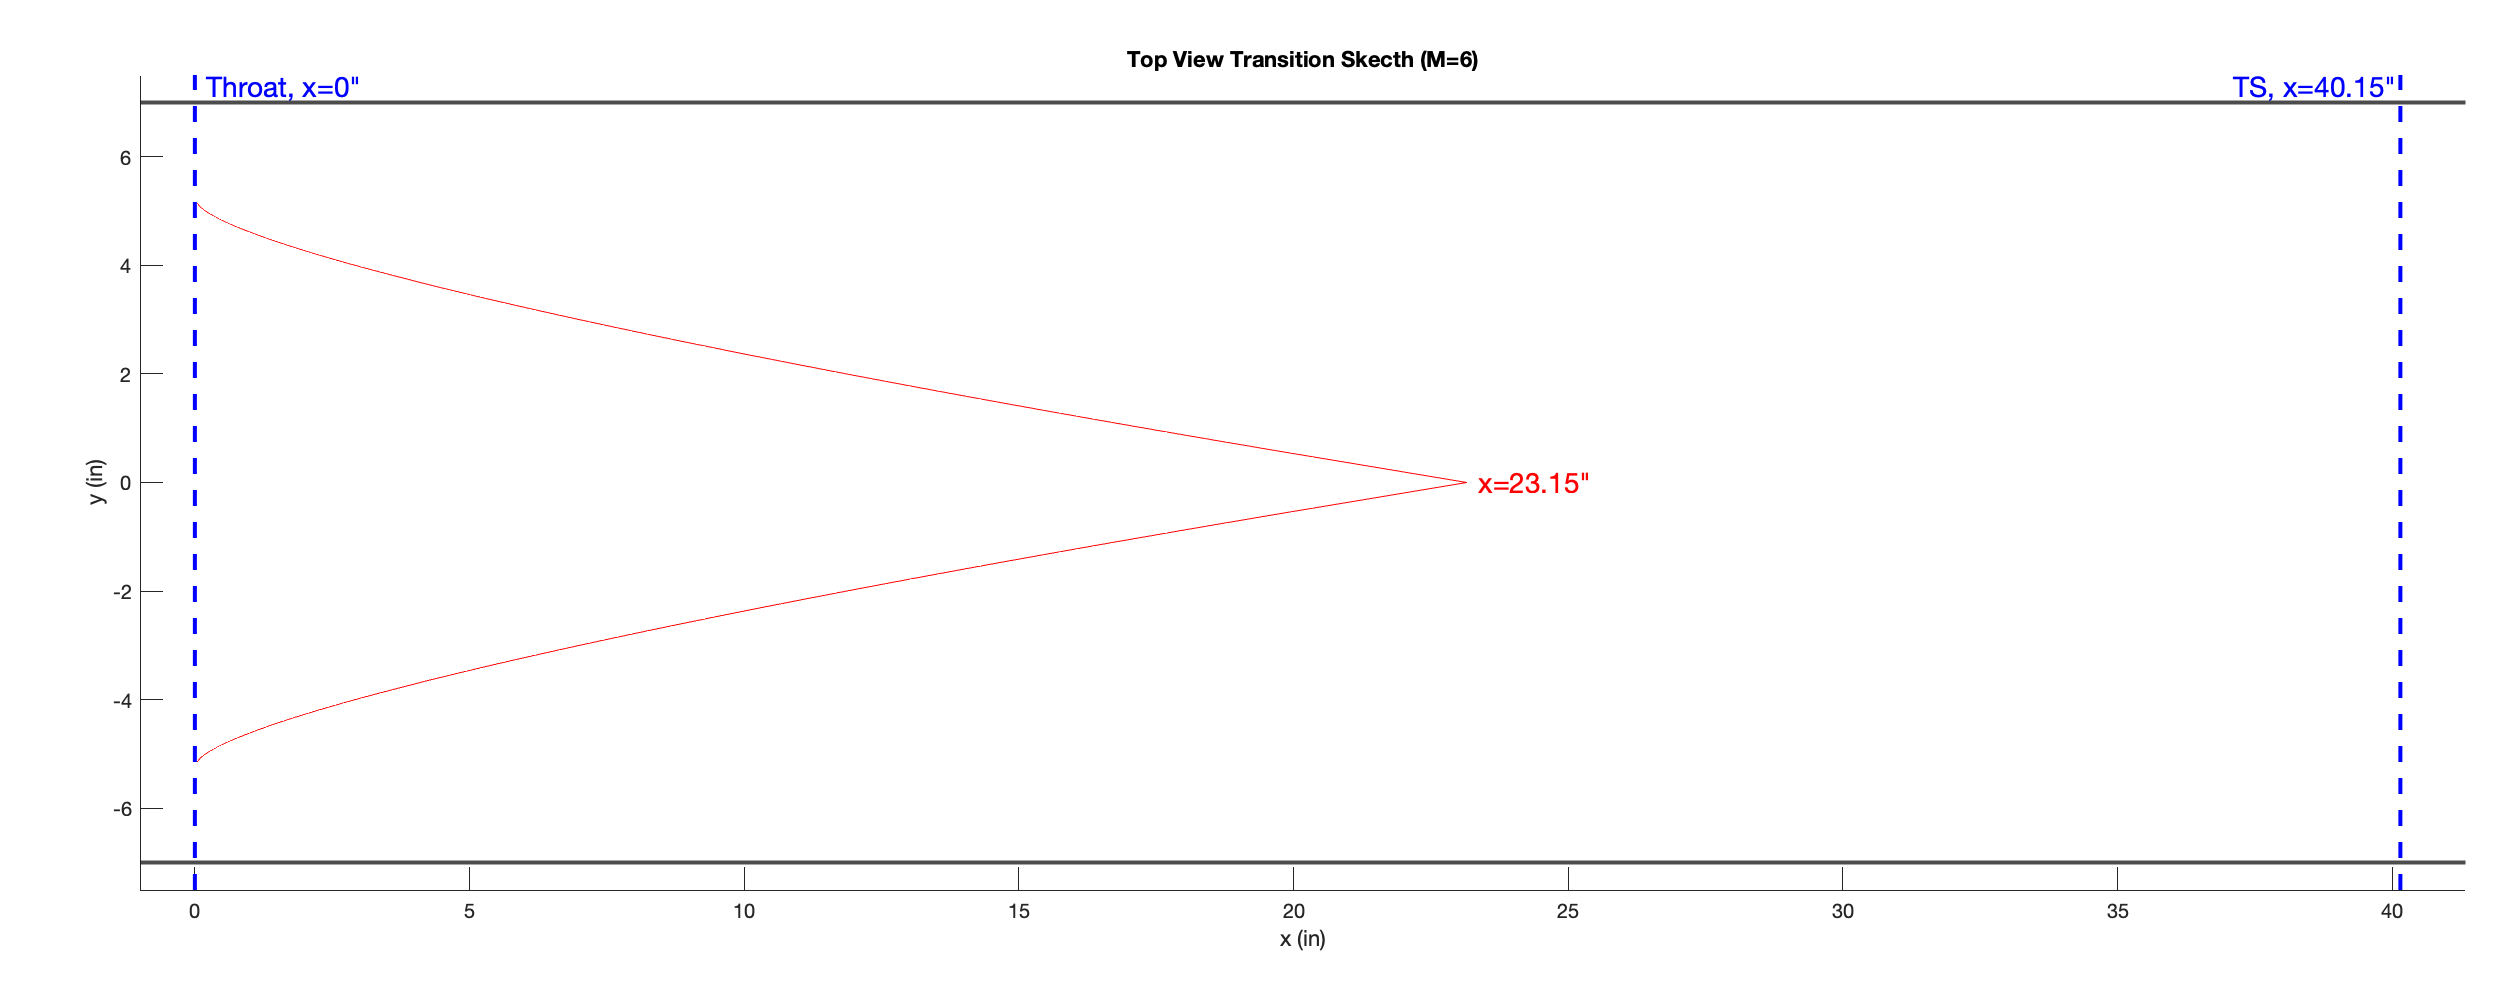
\includegraphics[width=6.5in]{top17}
    \caption{Mach lines for noise measured at 17" upstream on nozzle exit.}
    \label{fig:machlines}
\end{figure}

The above results reveal the pressure fluctuation levels increase but not the transition mechanism. The two primary suspects that can be eliminated using the data above are the sidewall mushroom vortices and Görtler vortices.

Sidewall mushroom vortices arise from the pressure distribution in the nozzle and the low momentum flow in the sidewall boundary layers. The flow at the centerline expands to the test section pressure ahead of the top and bottom curved walls. The flow at the top and bottom lags behind the centerline flow with a higher pressure to create a vertical pressure gradient that introduces a secondary vertical flow in the sidewall boundary layers that flows from the corners to the centerline \cite{sabnis}. CFD simulations show the sidewall mushroom vortices beginning to form approximately 24 inches upstream of the nozzle exit shown in Figures \ref{fig:mushrooms} and \ref{fig:vertical-vel}. Tracing the characteristics from 17 inches upstream of the test section entrance, Figure \ref{fig:machlines} shows the origin to be upstream of the throat where sidewall mushroom vortices are not relevant.

Görtler vortices are counter-rotating streamwise vortices that occur in boundary layers on concave surfaces \cite{saric}. To estimate where these may lead to transition, a CFD basic state simulation and N-factor analysis was performed by Kocian (2022). However, tracing the characteristics from 17 inches upstream of the test section entrance, Figure \ref{fig:machlines} shows the measured noise originates at the end of the straight section of the nozzle where Görtler is not relevant.

While both sidewall vortices and Görtler vortices can play some role in transition in planar nozzles, they are no longer considered suspects for the pressure fluctuation levels increase at unit Reynolds numbers above $3 \times 10^6 m^{-1}$.

The combination of pitot surveys and characteristic tracing eliminates the possibility of sidewall mushroom vortices or Görlter vortices because these instabilities would lead to transition downstream of the characteristic wall origins found by tracing from the measurement location to the wall intersection. This leaves the surface discontinuity at the throat as the primary culprit for the pressure fluctuation levels increase. The remaining suspect mechanisms are still important to note and address in the redesign of the ACE tunnel.

The following improvements are recommended to obtain laminar flow for some value above $Re' \approx 3 \times 10^6 m^{-1}$:
\begin{enumerate}
    \item Second-derivative-smooth subsonic-to-supersonic throat transition (eliminate discontinuity)
    \item Continuous curvature with analytical functions (eliminate waviness and discontinuities)
    \item Mirror polishing as much as possible (eliminate roughness/waviness)
    \item Improved settling chamber performance
    \item Subsonic boundary layer suction/bleed
\end{enumerate}

\subsection{Active Contol Capability}

Despite the intention of the ACE design, the mechanical realization does not allow for active contol. In fact, changing the Mach number at all is far from a simple process. 

\section{ACE2.0 Design}

Following the above conclusions and recommendations, the most likely reason the pressure fluctuations increase is laminar-to-turbulent transition due to a surface discontinuity at the throat. This conclusion is supported by pitot surveys, CFD, and method of characteristics line tracing described above. To correct this, the nozzle will be redesigned and remanufactured to meet specific requirements that will ensure the best performance and potentially expand the laminar Reynolds number range. The decision to remanufacture the nozzle presents an oppportunity to revise the nozzle and settling chamber design to achieve true active controllability, properly embodying ACE2.0 name.

The rest of the chapter details the planned improvements to the ACE tunnel and specific design requirements that will achieve those improvements. In addition to a new nozzle, the settling chamber will also be redesigned to improve the uniformity and turbulence of the incoming flow into the nozzle. These improvements are to achieve the goal of increasing the unit Reynolds number at which laminar nozzle flow is maintained.

\subsection{Design Requirments}

ACE2.0 shall maintain many characteristics while improving some, so many requirements are the same as the original ACE design. The new tunnel will still produce uniform Mach 5 to 8 flow in the 9 inches by 14 inches test section, withstand a 530 Kelvin total temperature, and maintain an engineering factor of safety of 4 when operating at a total pressure of 200 psi.

The overall improvements and associated requirements will be a new frame that will support a new actuation system with an efficient means of repeatably adjusting throat height to achieve desired mach numbers with a displacement indicator to achieve a repeatable Mach number change by 2 students in 4 hours or less, straightforward settling chamber and nozzle access for inspection and maintenance, and a rigid assembly for actuation between the settling chamber and nozzle.

\subsubsection*{Nozzle Requirements}

The current ACE nozzle successfully produces uniform Mach 5 to 8 flow in its core. In order to maintain this good performance and not introduce unknown parameters, the new nozzle will retain a very similar contour with slight improvements. The requirements that remain the same are that the nozzle must produce uniform flow for the entire Mach range, achieve maximum height deflection without damage, and prevent leaks up to a pressure of 200 psi.

The improvements to the nozzle and associated requirements will be a single-piece nozzle that eliminates any potential manufacturing discontinuities or steps, a contour with continuous 1st and 2nd derivatives that is specified by an analytical functions that will eliminate discontinuities and truncation error, and a maximum allowable stress less than or equal to that found in the current ACE flexure.

\subsubsection*{Settling Chamber Requirements}

The current ACE settling chamber design provides multiple opportunities to improve flow conditioning and ease of maintenance. The new settling chamber design will increase the length and height and allow for variable aerogrid/screen configurations. The requirements that remain the same are low freestream turbulence, thin stable wall boundary layers, maximum uniformity, and preventing leaks at a pressure of 200 psi. The implementation of these requirements will be improved in the new design to achieve improved incoming flow into the nozzle.

Following Reshotko \cite{reshotko}, the length of the settling chamber shall accommodate a separation of 250 characteristic mesh sizes between screens allowing for adequate turbulence decay. The aerogrids will have a hexagonal perforation pattern to increase porosity and decrease pressure loss. The number of aerogrids and screens shall be variable to allow for future flow conditioning experiments. The inlet shall include a baffle system that will provide an acceptable initial distribution of air received from the high-pressure inlet piping. The overall design shall accommodate future boundary layer suction or bleed slots.

A settling chamber height of 6" was chosen ... 10 ft/s to 100 ft/s Pope \cite{pope}:

\begin{table}[ht]
    \centering
    \label{tab:sc_vel}
    \begin{tabular}{|c|c|c|c|c|}
        \cline{2-5}
        \multicolumn{1}{c}{} & \multicolumn{4}{|c|}{\textbf{Mach Number}} \\ \hline
        \textbf{Height} & 5 & 6 & 7 & 8 \\ \hline
        4" & 73.57 & 34.55 & 17.64 & 9.66 \\ \hline
        5" & 58.83 & 27.64 & 14.11 & 7.73 \\ \hline \hline
        6" & 49.01 & 23.03 & 11.76 & 6.44 \\ \hline \hline
        7" & 42.00 & 19.74 & 10.08 & 5.52 \\ \hline
        8" & 36.75 & 17.27 & 8.82 & 4.83 \\ \hline
        9" & 32.66 & 15.35 & 7.84 & 4.29 \\ \hline
    \end{tabular}
    \caption{Settling chamber velocities (ft/s) for combinations of settling chamber heights and Mach numbers.}
\end{table}
    
\subsection{Nozzle Contour Codes}

The method-of-characteristics Fortran script written by Bowersox that produced the ACE nozzle contour was used for the new nozzle contour. In order to achieve continuous first and second derivative coninuity, a section of the code was modified to produce a fourth-order expansion section instead of the original second-order curve. This allowed the expansion section to match the curvature of both the subsonic section and the straight section.

\begin{singlespace}
    \textbf{Before}:

    \textit{do 10 i=1, nch}

    \textit{\; theta(i) = dthetai + float(i-1)*dth}

    \textit{\; x(i) = tan(theta(i))/2./k}

    \textit{\; xw(i) = x(i)}

    \textit{\; y(i) = 1.0 + k*x(i)**2}

    \textit{\; yw(i) = y(i)}

    \textit{10 continue}

    \textit{ }
    
    \textbf{After}:

    \textit{do 10 i=1, nch }

    \textit{\; theta(i) = dthetai + float(i-1)*dth}

    \textit{\; xthetai = sqrt(tan(thetai)/k)}

    \textit{\; k4 = -k/2./xthetai}

    \textit{\; pc = -9.*(k**2)/3./((4.*k4)**2)}

    \textit{\; qc = (2.*(3.*k)**3 - 27.*((4.*k4)**2)*tan(theta(i)))}

    \textit{\& \quad /27./((4.*k4)**3)}

    \textit{\; npi = 2.*pi/3.}

    \textit{\; tc = 2.*sqrt(-pc/3.)}

    \textit{\& \quad *cos(acos((3.*qc/2./pc)*sqrt(-3./pc))/3. - npi)}

    \textit{\; if((3.*qc/2./pc)*sqrt(-3./pc).lt.-1.) then}

    \textit{\; \qquad tc = 2.*sqrt(-pc/3.)*cos(acos(-1.)/3. - npi)}

    \textit{\; end if}

    \textit{\; x(i) = tc - k/4./k4}

    \textit{\; xw(i) = x(i)}

    \textit{\; y(i) = 1.0 + k*x(i)**3 + k4*x(i)**4}

    \textit{\; yw(i) = y(i)}

    \textit{10 continue}
\end{singlespace}

\begin{figure}[ht]
    \centering
    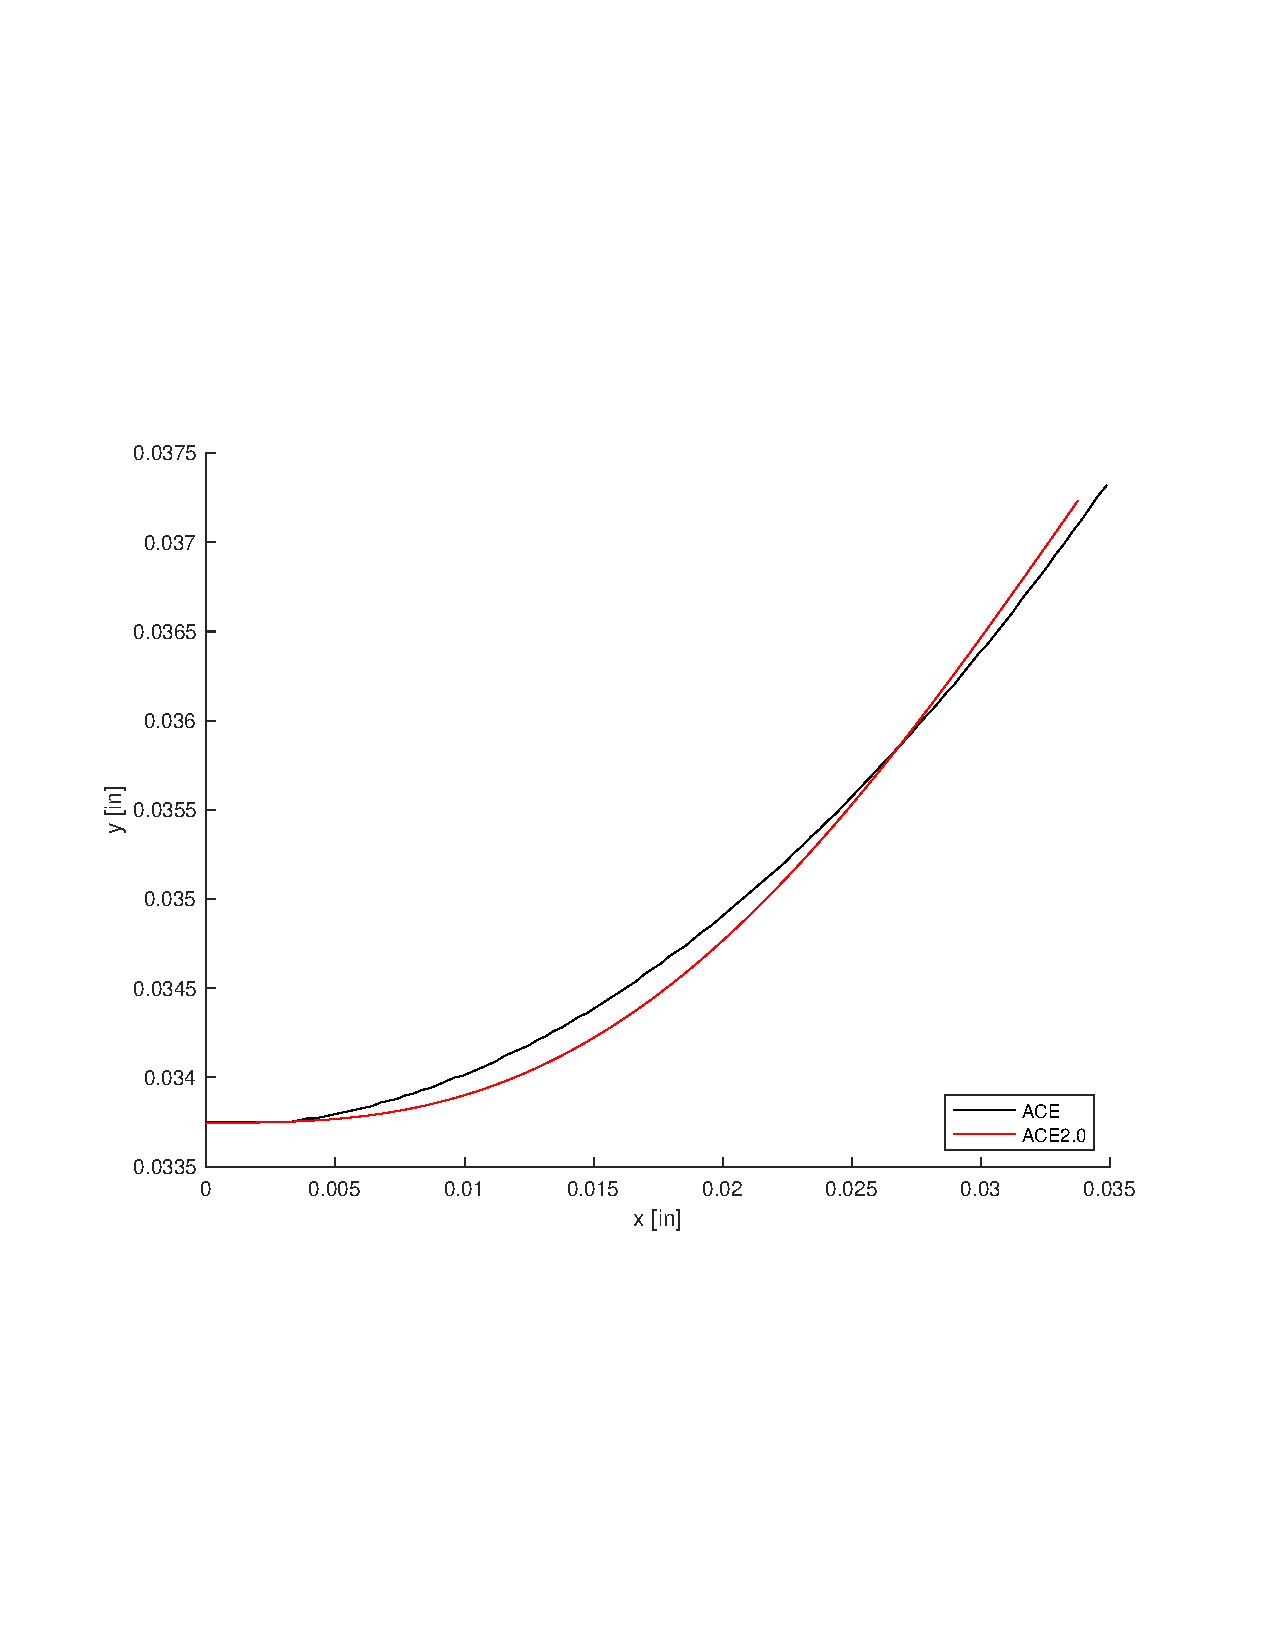
\includegraphics[width=6in]{throats}
    \caption{Comparison of ACE (quadratic) and ACE2.0 (quartic) expansion at throat}
    \label{fig:throats}
\end{figure}

After the points were produced by the Fortran script, they were imported into a MATLAB script to fit with analytic functions. 

Equations as follows:

\textbf{Subsonic:} $-0.0002679752287799994x^5 - 0.0066993807195x^4 - 0.04466253813x^3 + 0.033746187$ \textit{for} $-10 < x < 0$

\textbf{Throat:} $-2689.610971179115x^4 + 181.528229581324x^3 + 0.033746187$ \textit{for} $0 < x < 0.033746187$

\textbf{Straight:} $0.206725280364801x + 0.030258092015591$ \textit{for} $0.033746187 < x < 6.1460114$

\textbf{Straightening:} $2.180909737850381x^{0.960492634168194} + 5.934566177927477 \times 10^{284} x^{-367.9331632104439} - 0.585293189697896 - 1.684363604007221x^{1.011336503949665} - 0.023814395465567 \ln(0.418646933043039x)$ \textit{for} $6.1460114 < x < 40.07774$

\subsection{CFD}

In order to verify the above nozzle contour performance compared to the original ACE contour, both contours were simulated in 2-D with CFD. First, a mesh was created in Pointwise for each contour with 400 equally spaced columns of cells in the x-direction. Each column had the spacing scaled to accurately capture the boundary layer with the smallest cell height around 1e-5 meters at the curved wall and the largest around 0.1 meters at the centerline as seen in Figure \ref{fig:mesh}.

After creating a mesh for each, they were ran in US3D on the Texas A\&M supercomputer, GRACE. \textit{Stuff about inputs and convergence conditions}

\begin{figure}[ht]
    \centering
    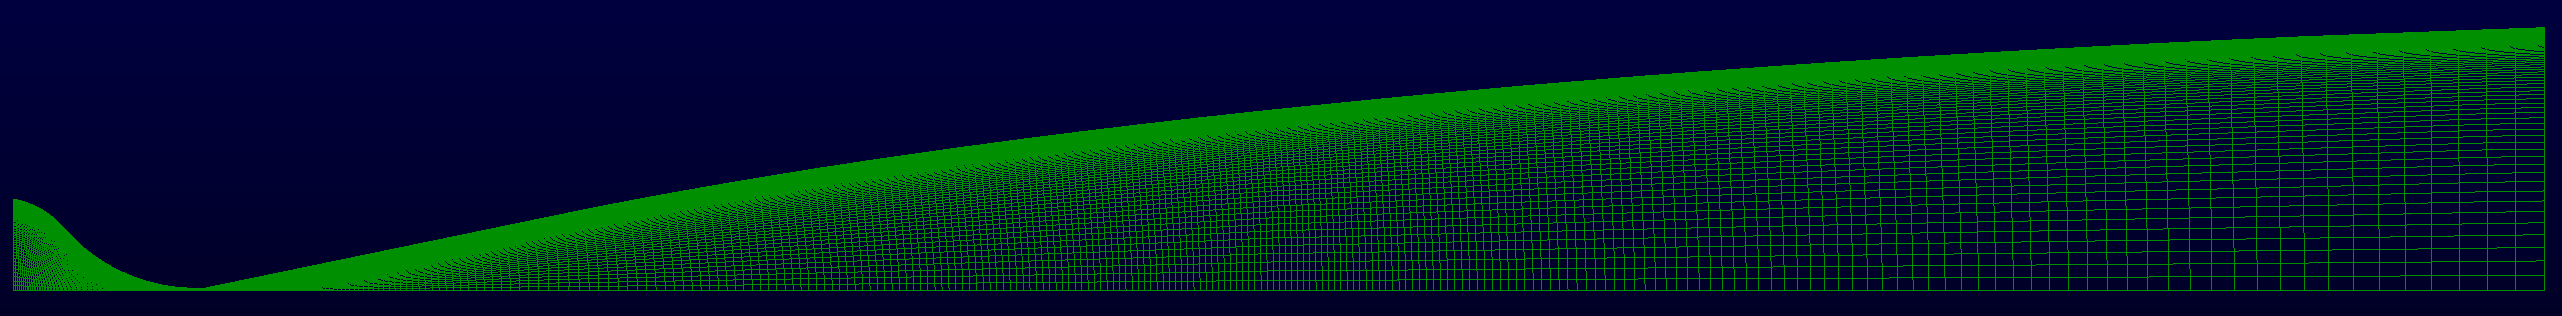
\includegraphics[width=6in]{ace-mesh}
    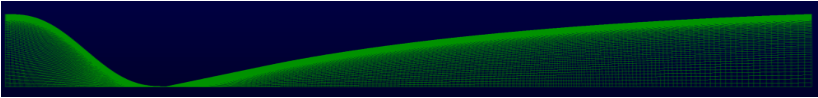
\includegraphics[width=6in]{qace-mesh}
    \caption{Mesh in Pointwise for ACE (top) and ACE2.0 (bottom) nozzle contours}
    \label{fig:mesh}
\end{figure}

\subsection{20-Ton Linear Actuators Design}

The updated ACE design follows the requirements above and is shown in the following figures. The new design exhibits an improved nozzle contour, settling chamber, and actuation design:
\begin{itemize}
    \item The overall length was increased by 16 inches to accommodate the much larger settling chamber.
    \item The actuation design consists of multiple worm gears to achieve a high gear ratio with minimal backlash. The Mach number can be changed quickly and accurately with a 0.005 inch throat height adjustment per control shaft rotation.
    \item The settling chamber exhibits inlet flow spreaders and an adaptable flow conditioner design.
    \item The nozzle is a single piece to eliminate any potential manufacturing steps and discontinuities.
    \item The stand will integrate with existing ACE infrastructure.
\end{itemize}

\subsubsection{Nozzle and Settling Chamber Design}

The nozzle and settling chamber are combined to accomodate active control.

The flow conditioners will be enclosed in a standalone box that can be modified or replaced easily.

The nozzle blocks will be made from 304 stainless steel, and the flexures will be made from 17-4 PH stainless steel.

\subsubsection{Frame Design}

Stuff and figures

Originally planned to water jet bars from brace stock to save material cost and reduce excess. Later discovered that the cost of time and tooling on water jet to cut all pieces from 3 inch 4140 allot steel exceeds the cost of ordering bar stock.

\subsubsection{Actuation System Design}

Detailed specifics of actuation components

\subsubsection{Final Overall Design}

Pictured below is the final overall ACE2.0 assembly.

\begin{figure}[ht]
    \centering
    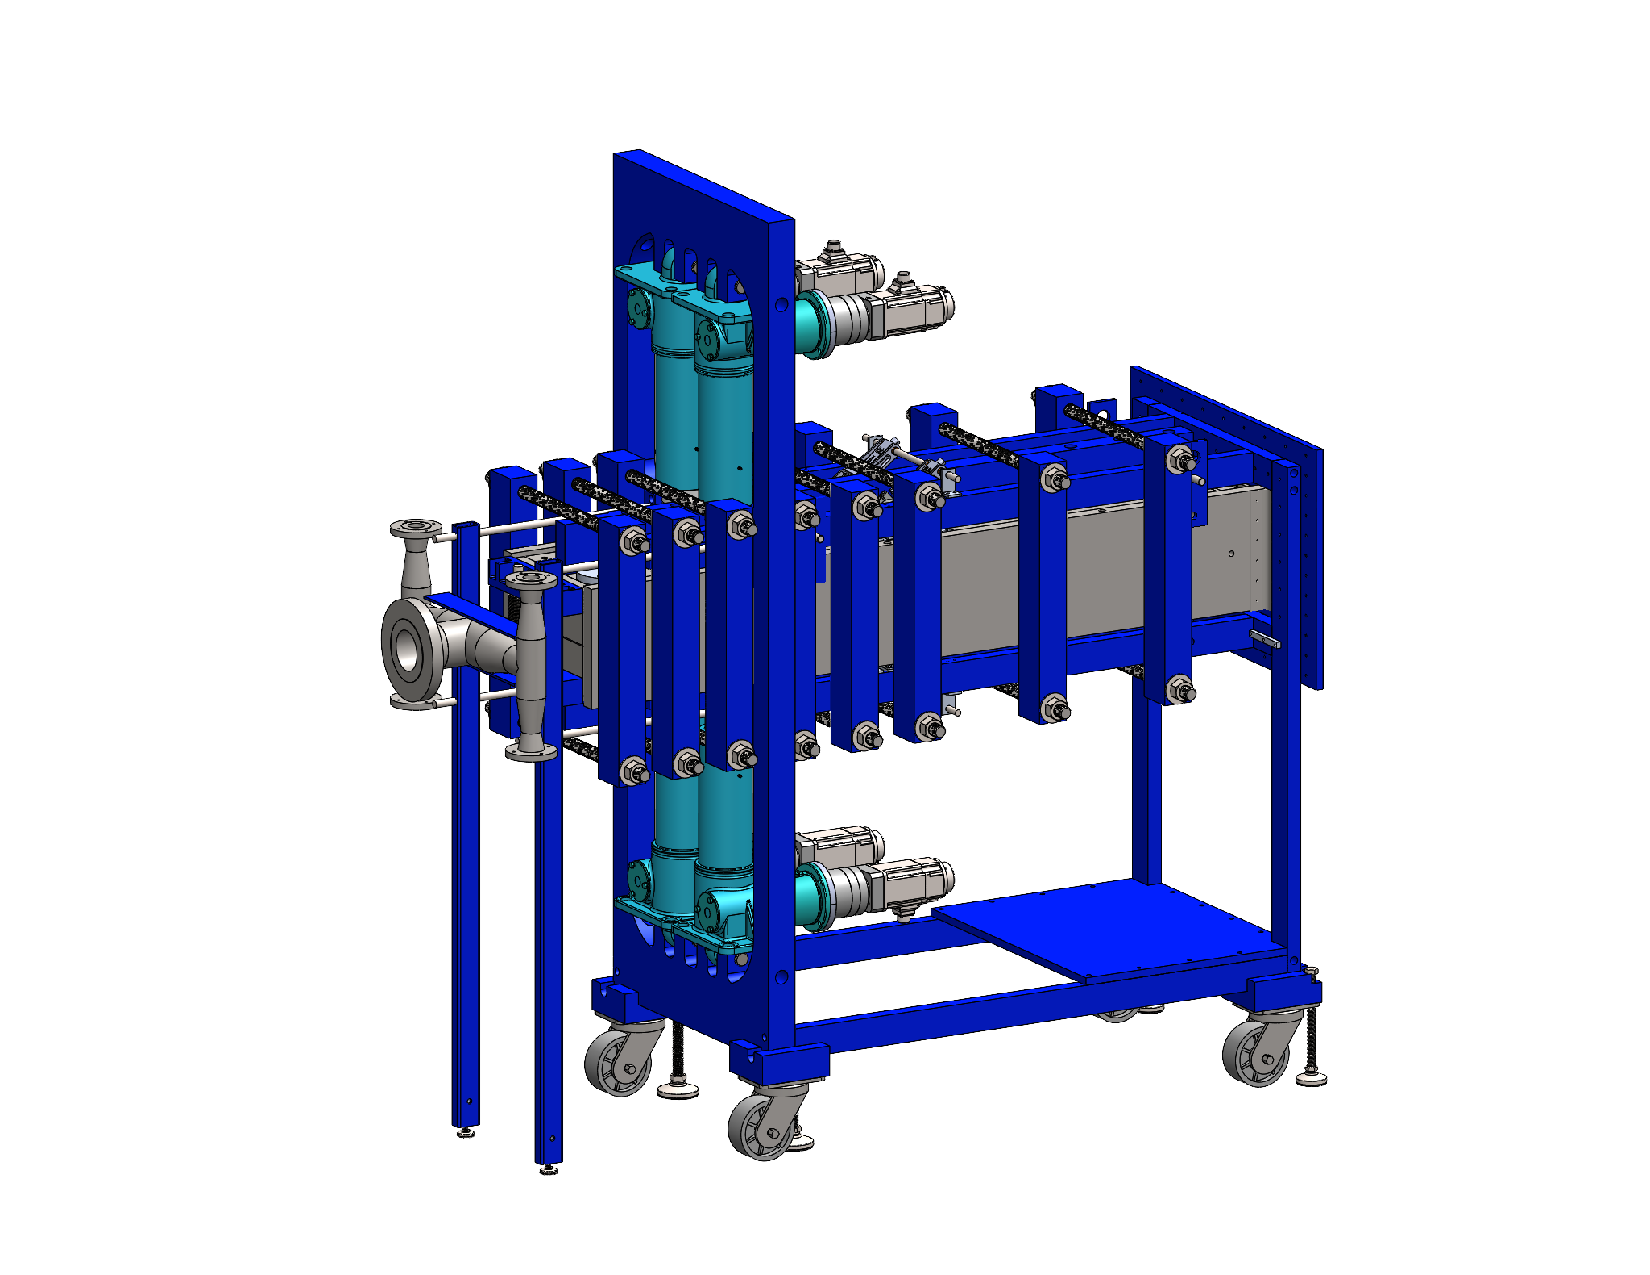
\includegraphics[width=6in]{cad-full}
    \caption{Temporary full CAD design}
    \label{fig:cad-full}
\end{figure}

\subsubsection{FEA}

Stress and FOS stuff with figures

\section{Fabrication Plans}

ACE2.0 is currently being fabricated. Most machining is completed. Pictures of machining and fabrication.

\subsection{Pressure Test}

Check structral integrity at 200 psia and evaluate sealing.

\subsection{Polishing}

Astro Pal polishing nozzles and sidewalls to 1 Ra.

\section{Final Assembly, Installation, and Calibration}

The final assembly will occur at NAL. Once nozzles and actuators are assembled in the frame, ACE2.0 will be rolled into the lab to replace ACE. All hoses, wires, and instrumentation attached to the nozzle and settling chamber will be removed and ACE will be rolled out of the lab. ACE2.0 will roll in and reconnect all hoses, wires, and instrumentation.

\subsection{Actuation Homing and Calibration}

Before the sidewalls are installed, the nozzles will be aligned by homing the servo motors with the limit switches. At this point shims will be used to make fine adjustments to limit switch positions to ensure a minimum Mach number of 4.9??? and a maximum Mach number of 8.5???.

\subsection{Shakedown and First Runs}

Decide what the first runs' purposes should be to properly calibrate.

